%!TEX root = JakubJedryszek-MasterThesis.tex

\cleardoublepage


\chapter{PCA Pump}
\label{pcapump}

% http://www.santoslab.org/pub/paper/LarsonEtAl13-PCA-Requirements-SEHC-preprint.pdf
% http://ppahs.org/2012/05/30/patient-controlled-analgesia-pca-pumps-the-basics/

\begin{wrapfigure}{r}{0.4\textwidth}
  \begin{center}
    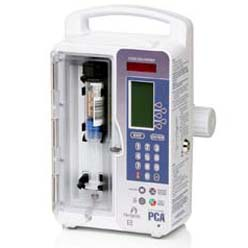
\includegraphics[width=0.4\textwidth]{figures/pca-pump.png}
  \end{center}
  \caption{Patient Controlled Analgesia (PCA) pump}
  \label{figure:pca-pump}
\end{wrapfigure}

Patient Controlled Analgesia (PCA) pump is a medical device, which allows the patient to self-administer small doses of narcotics (usually Morphine, Dilaudid, Demerol, or Fentanyl). PCA pumps are commonly used after surgery to provide a more effective method of pain control than periodic injections of narcotics. A continuous infusion (called a basal rate) permits the patient to receive a continuous infusion of pain medication. There is no need for a clinician to administer it. Patient can also request additional boluses, but only in specified intervals. It prevents from over infusion. In addition to basal and patient bolus, clinician can also request bolus called clinician bolus or square bolus. 

Figure \ref{figure:pca-pump} shows LifeCare PCA pump. On the left hand side, there is drug reservoir. On the right -  clinician panel, which allows to control the pump. Figure \ref{figure:alaris-pump} shows PCA Pump, made by company Alaris. 

\begin{wrapfigure}{l}{0.4\textwidth}
  \begin{center}
    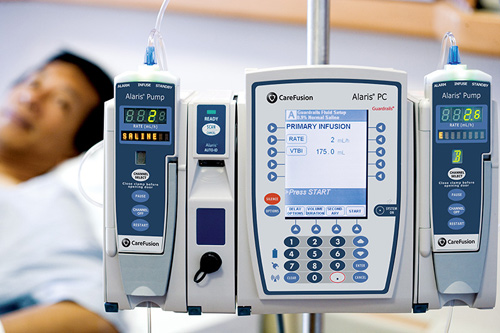
\includegraphics[width=0.4\textwidth]{figures/alaris-pump.png}
  \end{center}
  \caption{Alaris Pump}
  \label{figure:alaris-pump}
\end{wrapfigure}

PCA Pump is safety-critical device which works in standard process control loop depicted in the Figure \ref{figure:control-loop}. The controller obtains information about (observes) the process state from measured variables (feedback) and uses this information to initiate action by manipulating controlled variables to keep the process operating within predefined limits or set points (the goal) despite disturbances to the process. Such as different air pressure or device position (gravity impact). In general, the maintenance of any open-system hierarchy (either biological or man-made) will require a set of processes in which there is communication of information for regulation or control \cite{SaferWorld}.

\begin{figure}[ht]%t=top, b=bottom, h=here
    \begin{center}
    	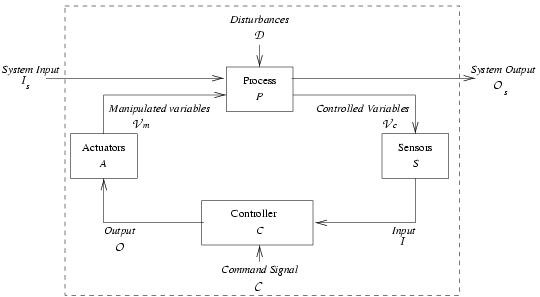
\includegraphics[width=0.9\textwidth]{figures/safety-critical-loop.png}    	
    \end{center}
    \caption{Standard Process Control Loop.}
    \label{figure:control-loop}
\end{figure}

PCA Pump actuator is motor, which pump drug to the patient's vein. Controlled process is dosing the drug. Sensors measure amount of dosed drug. They might be used for double-check if ordered (by controller) amount of drug was appropriately delivered. Sometimes there might be some distrubances caused by mechanical issues and environmental conditions. Controller issues appropriate actions based on information from sensors and clinician or patient's commands. High level overview of PCA Pump is depicted in the Figure \ref{figure:pca-pump-system}.

\begin{figure}[ht]%t=top, b=bottom, h=here
    \begin{center}
    	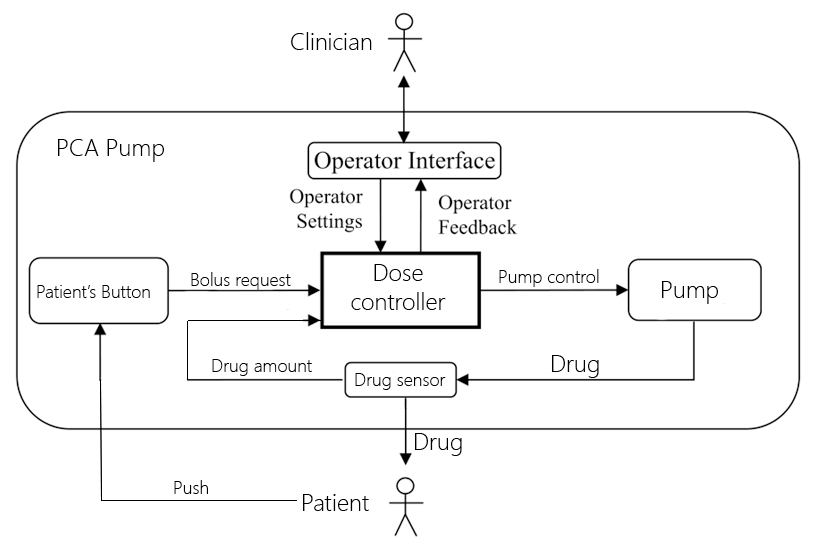
\includegraphics[width=0.9\textwidth]{figures/pca-pump-system.png}    	
    \end{center}
    \caption{PCA Pump system}
    \label{figure:pca-pump-system}
\end{figure}

One of the hazards of using PCA pumps, is that there is inadequate monitoring of patient's levels of oxygen and carbon dioxide. Nursing staff on general medical units typically track respiration rate and other vital signs every four hours, which is not enough. There should be a way to monitor levels continuously. Additionally, it can be hard to tell if a person's breathing rate is dangerously low in certain circumstances. There are cases, where lack of monitoring carbon dioxide level caused death.\footnote{http://abcnews.go.com/Health/parents-warn-pca-pumps-daughters-death/story?id=16796805} 

Another hazard is human mistake. For example, there is a case when nurse used a 5 mg/mL morphine cassette because a 1 mg/mL cassette was not available, but she programmed PCA Pump like for 1 mg/mL concentration. In addition to lack of monitoring of the pulse, patient died.\footnote{http://webmm.ahrq.gov/case.aspx?caseID=291}

As mentioned in chapter \ref{background}, the solution to that problem is medical devices interoperability. In addition, less human error-prone device is needed. It can be assured by using more than one system for their detection.



\section{PCA Pump Requirements Document}
\label{pcapump:requirements-doc}

Requirements of "Open Source PCA Pump" \cite{OpenSourcePCAPump:Paper} are captured in "Open Patient-Controlled Analgesia Infusion Pump System Requirements" document \cite{PcaReq} created by Brian Larson. It is formalized set of capabilities, which Open PCA Pump should have, based on consultations with domain experts, FDA and Brian Larson's expertise gained while he was working in the medical device industry.

Conceptual model of Open PCA pump is depicted in the Figure \ref{figure:ice-pca-pump}. As mentioned earlier, the pump is connected to ICE so it may be integrated with ICE apps and displays. The interface must provide prescription and patient information, current status to be displayed remotely on a supervisor user interface, and a means to stop infusing upon human command, or determination of an ICE app. Such an ICE app could monitor a patient's blood oxygenation and pulse rate, stopping the pump if depressed respiratory function is indicated \cite{PcaReq}.

\begin{figure}[ht]%t=top, b=bottom, h=here
    \begin{center}
      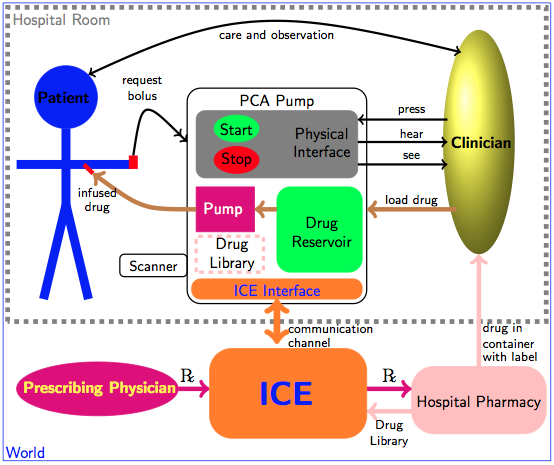
\includegraphics[width=0.9\textwidth]{figures/ice-pca-pump.png}      
    \end{center}
    \caption{Open PCA Pump concept}
    \label{figure:ice-pca-pump}
\end{figure}

Additionally, it cooperates with Drug Library, which contains information about drugs and its properties (like concentration). Data needed for pump operation, are captured on electronic prescription, which contains:
\begin{itemize}
    \item Patient's name
    \item Drug name
    \item Drug code
    \item Drug concentration
    \item Initial volume of drug in the vial
    \item Basal flow rate - the rate of continuous infusion
    \item Volume to be infused (VTBI) on patient's request
    \item Maximum amount of drug allowed per hour
    \item Minimum time between patient boluses
    \item Date, in which prescription has been filled
    \item Prescribing physician's name
    \item Pharmacist name
\end{itemize}

Pain medication is prescribed by a licensed physician, which is dispensed by the hospital's pharmacy. The drug is placed into a vial labeled with the name of the drug, its concentration, the prescription, and the intended patient. A clinician loads the drug into the pump, and attaches it to the patient. The pump infuses a prescribed basal flow rate which may be augmented by a patient-requested bolus or a clinician-requested bolus. This allows additional pain medication in response to patient need within safe limits \cite{PcaReq}.

Prescription captures all data needed for basal infusion and patient requested boluses (referred as bolus). In addition to that, Open PCA Pump allows Clinician Requested Bolus (refereed as square bolus). In order to do that, clinician has to enter the time (through PCA Pump panel) in which VTBI, specified in prescription, will be infused.

There can occur situations in which the maximum drug amount infused may exceed the allowed limit. E.g. when clinician issues too many square boluses. In such case, pump is switched to Keep Vein Open (KVO) mode, which has 1 ml/hr drug rate. Pump switches to KVO rate also when ICE interface request it. It may happen e.g. if patient's oxygen level is low. To recover from KVO state, pump has to be restarted by clinician in order to continue operation. In Summary, Open PCA Pump has following modes:
\begin{itemize}
    \item Stopped
    \item Basal rate
    \item Patient's bolus (bolus)
    \item Clinician bolus (square bolus)
    \item Keep Vein Open (KVO)
\end{itemize}

There are also other scenarios, which are captured by Requirements Document \cite{PcaReq}, like scanner to enable automatic entry of patient's and prescription data, occlusion detection, hardware errors alarms etc. Detailed overview of Open PCA Pump Requirements can be found in \cite{PcaReq}.




\section{PCA Pump AADL/BLESS Models}
\label{pcapump:aadl-bless-models}

In addition to PCA Pump Requirements Document \cite{PcaReq}, Brian Larson created AADL model with formal behavioral specifications written in his BLESS framework. AADL model, graphical representation is depicted in the Figure \ref{figure:pca-pump-aadl-model}. 

\begin{figure}%[h]%t=top, b=bottom, h=here
    \begin{center}
      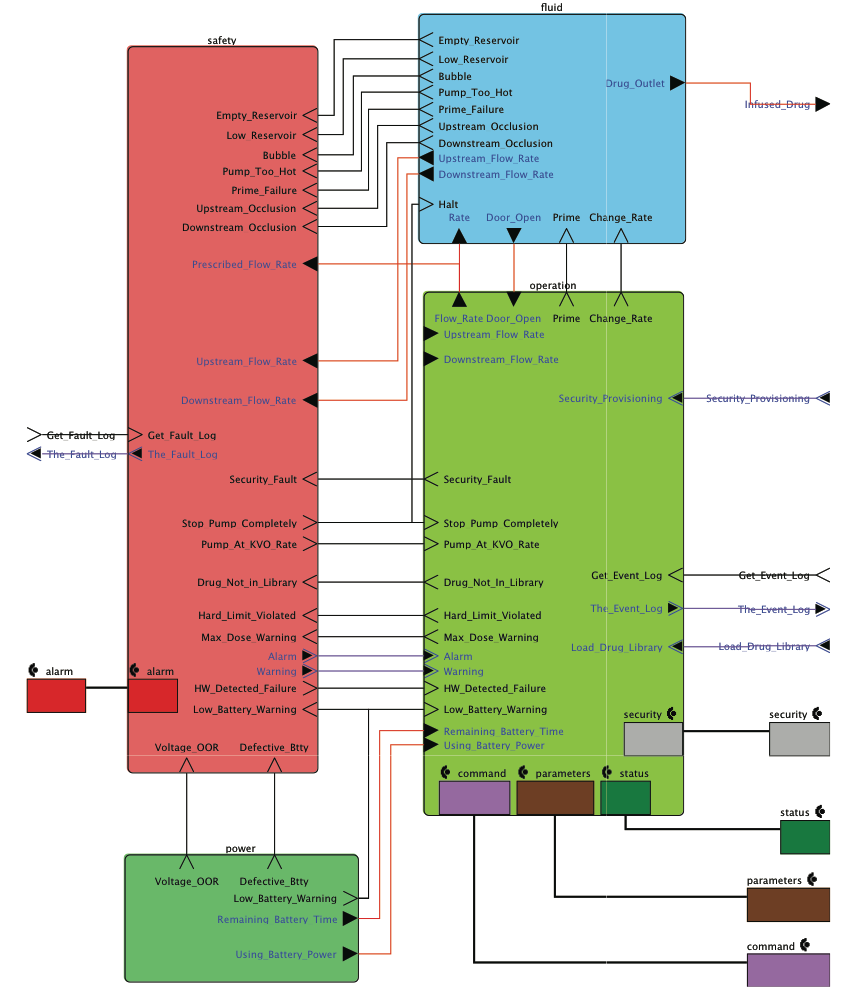
\includegraphics[width=0.9\textwidth]{figures/pca-pump-aadl-model.png}      
    \end{center}
    \caption{Open PCA Pump AADL model}
    \label{figure:pca-pump-aadl-model}
\end{figure}

AADL model captures structure of device. BLESS - its behavior. In appendix \ref{Appendix:AADL:RateController}, thread \lstinline{Rate_Controller} from \lstinline{PCA_Operation} component with BLESS assertions in thread declaration and BLESS behavioral description in thread implementation, is presented. The thread declaration contains input and output ports. In addition to some of them, BLESS assertions are present. Assertions are defined in BLESS annex in thread implementation. In addition to assertions, states and transitions defined in thread implementation can potentially be translated into working SPARK Ada program. Presence of timing properties in states and transitions makes translation extremely difficult, thus there are omitted in this thesis and only assertions are considered.


\section{BeagleBoard-xM}
\label{pcapump:beagleboard}

\begin{wrapfigure}{r}{0.5\textwidth}
  \begin{center}
    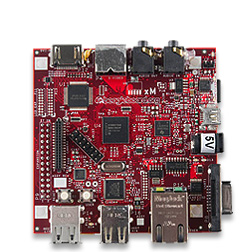
\includegraphics[width=0.5\textwidth]{figures/beagleboard_xm.png}
  \end{center}
  \caption{BeagleBoard-xM}
  \label{figure:beagleboard_xm}
\end{wrapfigure}

For Research and MDCF purposes, BeagleBoard-xM (an open-source hardware single-board computer produced by Texas Instruments), has been chosen as hardware platform for PCA pump prototyping.

BeagleBoard-xM (presented in the Figure \ref{figure:beagleboard_xm}) is Embedded device with AM37x 1GHz ARM processor (Cortex-A8 compatible). It has 512 MB RAM, 4 USB 2.0 ports, HDMI port, 28 General-purpose input/output (GPIO) ports and Linux Operating System (on microSD card). Moreover there is PWM support, which enables control of pump actuator.

Pulse-width modulation (PWM) is a technique for controlling analog circuits with a processor's digital outputs. The average value of voltage (and current) fed to the electrical load is controlled by turning the switch between supply and load on and off at a fast pace. The longer the switch is on compared to the off periods, the higher the power supplied to the load. Proportion of on and off periods is called the duty cycle and is expressed in percent. 100\% means all the time on, 0\% - all the time off. Figure \ref{figure:pwm} shows 10\%, 30\%, 50\% and 90\% duty cycles.

\begin{figure}[ht]%t=top, b=bottom, h=here
    \begin{center}
      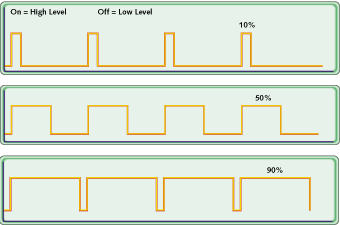
\includegraphics[width=0.9\textwidth]{figures/pwm.png}      
    \end{center}
    \caption{An example of PWM duty cycles}
    \label{figure:pwm}
\end{figure}

There is no existing SPARK Ada compiler running on ARM system. Hence, to compile SPARK Ada program for ARM device, cross-compiler is needed. There is GNAT compiler \cite{Horn:Thesis} created by AdaCore, but there was no cross-compiler for ARM. However, AdaCore was actively developing cross-compiler. They had working version in 2013, but tested only on their target Android-based device. In cooperation with AdaCore, cross-compiler for ARM was bundled and tested on BeagleBoard-xM. For now, GNAT cross-compiler works only on Linux 32-bit operating system.

In addition to USB ports, BeagleBoard-xM has also serial port and Ethernet port. It allows to copy programs compiled on Linux, using all three types of ports. 
